\documentclass{article}
\usepackage[utf8]{inputenc}
\usepackage[margin=1in]{geometry} % Keeps margins tight for 1-page fit
\usepackage{graphicx}
\usepackage{float} % Required for the [H] figure placement
\title{Report.1.Gradient.descend}
\author{Karma}
\date{May 2026}

\begin{document}

\maketitle

\section{Inplement}
To implement the algorithm i first create a function f(x) that returns $\mathbf{x^2}$

Then create a function df(x) that returns 
$\mathbf{2*x}$.

To calculate the gradient descent, i use this formula: 
$\mathbf{x = x - L * df(x)}$
with L is the learning rate (in this exercise i set it equal to 0.1)

The result looks like: 
\begin{figure}[H]
    \centering
    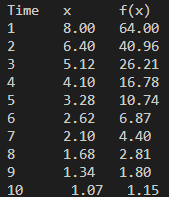
\includegraphics[width=0.25\linewidth]{images/lr0.1.png}
    \caption{With learning rate = 0.1}
    \label{fig:placeholder}
\end{figure}

With learning rate = 1, it can not go to the minimum value
\begin{figure}[H]
    \centering
    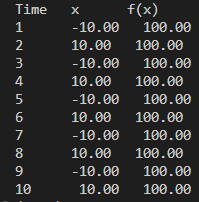
\includegraphics[width=0.25\linewidth]{images/lr1.png}
    \caption{With learning rate = 1}
    \label{fig:placeholder}
\end{figure}

With learning rate = 1, it converges very slow 
\begin{figure}[H]
    \centering
    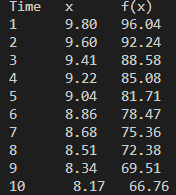
\includegraphics[width=0.25\linewidth]{images/lr0.01.png}
    \caption{With learning rate = 0.01}
    \label{fig:placeholder}
\end{figure}
\section{Observation}
The learning rate is too large that can lead to the unaccessable to the minimum point. The learning rate is too small can lead to the slow convergence. 

So the best way is to choose the learning rate = 0.1
\end{document}
